
\begin{lemma}
	Пусть $M$ -- гладкое многообразие в $\R^n$ и $f : M \to \R^m$. Следующие условия эквивалентны:
	\begin{enumerate}[itemsep = 0pt, topsep = 5pt]
		\item Отображение $f$ гладкое по Милнору,
		\item $\forall p \in M$ и любой параметризации $\phi : V \to \R^n$ в окрестности $p$ отображение $f \circ \phi : V \to \R^m$ гладкое (в обычном смысле),
		\item $\forall p \in M$ найдется параметризация $\phi : V \to \R^n$ в окрестности $p$, что отображение $f \circ \phi : V \to \R^m$ гладкое (в обычном смысле).
	\end{enumerate}
\end{lemma}

\begin{myproof}
	$(1 \Ra 2)$ Пусть $\phi : V \to \R^n$ -- параметризация $M$ в окрестности $p \in M$. 
	Рассмотрим гладкое продолжение $F$ функции $f$ в окрестности $p = \phi(a)$, $a \in V$. 
	Тогда $f \circ \phi = F \circ \phi$ в некоторой малой окрестности $a$. 
	Следовательно, $f \circ \phi$ гладкая в точке $a$ как композиция гладких функций $F$, $\phi$. 

	\vspace{5pt}
	$(2 \Ra 3)$ Это утверждение логически очевидно.

	\vspace{5pt}
	$(3 \Ra 1)$ Для $p \in M$ на $M \cap W$ мы можем записать равенство $f = (f \circ \phi) \circ \phi^{-1}$ (множество $M \cap W$ из определения параметризации, чтобы карта была определена). 
	Так как это верно $\forall p \in M$ и карта гладкая по лемме 3.1, то $f$ является гладкой на $M$ как композиция.
\end{myproof}

\begin{note}
	Пусть $M \subset \R^n$ и $N \subset \R^l$ -- гладкие многообразия и $f : M \to \R^l$ -- гладкое отображение, такое что $f(M) \subset N$. 
	Если $\phi$ и $\psi$ -- параметризации многообразий в окрестностях $p$ и $f(p)$ соответственно,
	то отображение $\psi^{-1} \circ f \circ \phi$ называется \textit{координатным представлением $f$ в окрестности $p$}. 
	Если $N$ открыто в $\R^l$, то $\psi$ полагаем равным $\id$.
\end{note}

\begin{example}
	Пусть $\gamma$ -- гладкая кривая на многообразии $M$ в $\R^n$, то есть 
	$\gamma : I \to \R^n$, $\gamma(I) \subset M$, $I$ открытый интервал и $\gamma$ гладкая.
	Если $p \in \gamma(I)$ и $\phi : V \to \R^n$ локальная параметризация $M$ в окрестности $p$, то $\beta = \phi^{-1} \circ \gamma$ является координатным представлением $\gamma$ в окрестности $p$. 
	Таким образом, на гладкую кривую $\gamma$ можно смотреть локально как на образ гладкой кривой $\beta$ под действием $\phi$.  
\end{example}


\subsection{Касательное пространство к многообразию}

\begin{definition}
	Пусть $M$ -- гладкое $m$-мерное многообразие в $\R^n$, $p \in M$. 
	Вектор $v \in \R^n$ называется \textit{касательным вектором} к $M$ в точке $p$, если найдется гладкая кривая $\gamma : (-\delta, \delta) \to M$, такая что $\gamma(0) = p$ и $\gamma'(0) = v$. 
	Множество касательных векторов к $M$ в точке $p$ обозначается $T_p M$ и называется \textit{касательным пространством} к $M$ в $p$.
\end{definition}

\vspace{-15pt}

\begin{figure}[h!]
\centering
\begin{framed}
		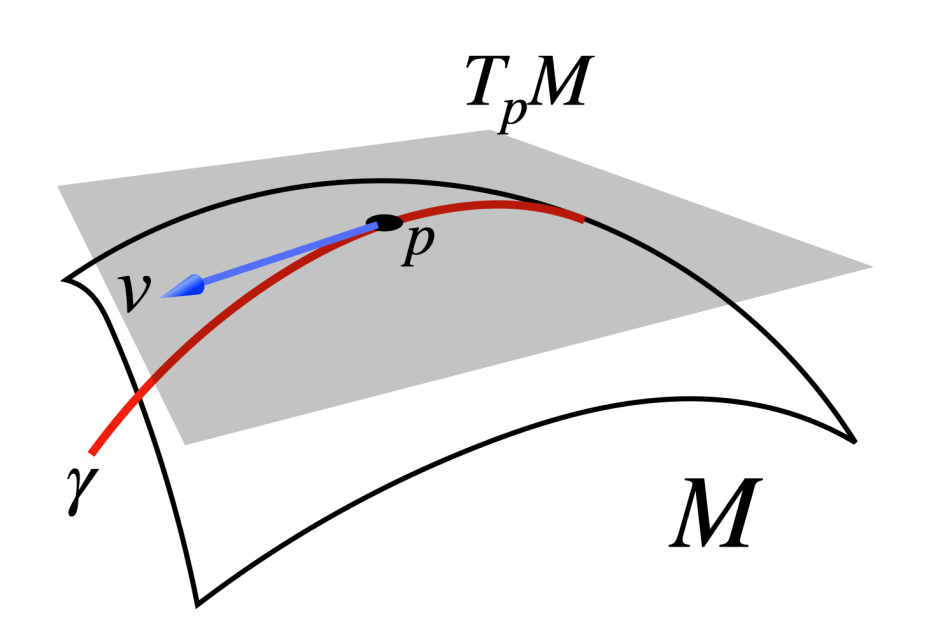
\includegraphics[width=0.3\textwidth, ]{Pictures/TpM.png}
		\caption{\raggedright Иллюстрация касательного пространства.}
		\label{fig:TpM}
\end{framed}
\end{figure}

\vspace{-15pt}

\begin{theorem}
	Пусть $M$ -- гладкое $m$-мерное многообразие в $\R^n$, $p \in M$. 
	Справедливы следующие утверждения: 
	\begin{enumerate}[itemsep = 0pt, topsep = 5pt]
		\item Если $\phi : V \to \R^n$ -- параметризация $M$ в окрестности $p = \phi(a)$, то $T_p M =  d \phi_a (\R^m)$,
		\item Пусть $U \ni p, W$ открыты в $\R^n$ и $\Phi : U \to W$ -- такой диффеоморфизм, что $\Phi(M \cap U) = W \cap (\R^m \times \{0\})$.
		Тогда $T_p M = (d \Phi_p)^{-1} (\R^m \times \{0\})$ ($= d (\Phi^{-1})_{\Phi(p)} (\R^m \times \{0\})$).
		\item Пусть $U \ni p$ открыто в $\R^n$ и гладкая функция $F : U \to \R^{n-m}$ такова, что $M \cap U = F^{-1}(0)$ и $\operatorname{rk} DF = n-m$ на $M \cap U$.
		Тогда $T_p M = \ker DF_p$.
	\end{enumerate}
\end{theorem}

\begin{myproof}
	Пусть $\phi : V \to \R^n$ -- функция из первого пункта, а диффеоморфизм $\Phi : U \to W$ из второго. 
	Покажем, что $d \phi_a (\R^m) \subset T_p M \subset d \Phi^{-1}_p (\R^m \times \{0\})$. 

	\vspace{5pt}
	Пусть $h \in \R^m$. Покажем, что $d \phi_a(h) \in T_p M$. Рассмотрим $B_r (a) \subset V$
	и выберем $\delta > 0$, что $\delta |h| < r$, тогда $a + th \in V$ для всех $|t| < \delta$.
	Определим $\gamma(t) = \phi(a + th)$, $t \in (-\delta, \delta)$. 
	Тогда $\gamma : (-\delta, \delta) \to M$ гладкая кривая, $\gamma(0) = \phi(a) = p$, $\gamma'(0) = d \phi_a (h)$, то есть $d \phi_a (h) \in T_p M$. 

	\vspace{5pt}
	Пусть $v \in T_p M$. Тогда $\exists \gamma : (-\delta, \delta) \to M$, $\gamma(0) = p$, $\gamma'(0) = v$. 
	Уменьшая $\delta$, если необходимо, можно считать, что $\gamma((-\delta, \delta)) \subset M \cap U$. 
	Следовательно, $\Phi(\gamma(t)) \in \R^m \times \{0\}$ при $|t| < \delta$, а значит, $d \Phi_p (v) = d \Phi_{\gamma(0)} (\gamma'(0)) = \frac{d}{dt}|_{t=0} \ \Phi(\gamma(t)) \in \R^m \times \{0\}$, 
	то есть $v \in (d \Phi_p)^{-1}(\R^m \times \{0\})$. 
	
	\vspace{5pt}
	Поскольку $d \phi_a$, $d \Phi^{-1}_p$ инъективны из максимальности ранга параметризации и невырожденности матрицы Якоби диффеоморфизма, то $d \phi_a(\R^m)$ и $d \Phi^{-1}_p(\R^m \times \{0\})$ -- линейные $m$-мерные пространства в $\R^n$. 
	Поэтому $T_p M$ совпадает с каждым из этих пространств. 

	\vspace{5pt}
	Установим третий пункт. Пусть $v \in T_p M$, тогда $\exists \gamma : (-\delta, \delta) \to M$, $\gamma(0) = p$, $\gamma'(0) = v$. 
	Можно считать, что в некоторой окрестности $t = 0$ выполнено $F(\gamma(t)) \equiv 0$, уменьшив $\delta$, если необходимо. 
	Продифференцируем тождество при $t = 0$. 
	Тогда $d F_{\gamma(0)} (\gamma'(0)) = 0 \Leftrightarrow d F_p (v) = 0 \Leftrightarrow v \in \ker DF_p$. 
	Откуда $T_p M \subset \ker DF_p$ и равенство пространств следует из совпадения размерностей: $m = \dim T_p M = \dim \ker DF_p$. 
\end{myproof}

\vspace{5pt}
Пользуясь известными фактами из алгебры, получим несколько следствий.

\begin{corollary}
	Отображение $d \phi_a : \R^m \to \im d \phi_a = T_p M $ задает линейный изоморфизм.
\end{corollary}

\begin{note}
	Пусть $(u_1, \dotsc, u_m)$ -- координаты в $\R^m$, тогда $d\phi_a(e_1), \dotsc, d\phi_a(e_m)$ или, что эквивалентно, $\frac{\partial \phi}{\partial u_1}(a), \dotsc, \frac{\partial \phi}{\partial u_m}(a)$ образуют базис в $T_p M$. 
	Если $h = (h_1, \dotsc, h_m) \in \R^m$, то по линейности $d \phi_a (h) = \sum \limits_{i=1}^{m} \frac{\partial \phi}{\partial u_i}(a) h_i$.
	Тогда $h_i$ являются координатами $d \phi_a(h)$ в базисе $T_p M$.
	
	Зафиксируем некоторый касательный вектор $v = d \phi_a(h)$ с кривой $\gamma$. Вспомним, что для некоторой кривой $\beta$ имеем $\beta = \phi^{-1} \circ \gamma \Leftrightarrow \gamma = \phi \circ \beta$, тогда $\gamma'(0) =  d \phi_{\beta(0)} (\beta'(0)) \Leftrightarrow d \phi_a(h) = d \phi_a (\beta'(0))$, поэтому $h = \beta'(0)$.
	Таким образом, векторы скорости из пространства параметров переходят в векторы скорости касательного пространства.
\end{note}

\begin{corollary}
	Если $M$ локально задано уравнением $F(x) = 0$, то есть $F$ из третьего пункта теоремы, $F = (F_1, \dotsc, F_{n-m})$, то 
	$T_p M = \ker DF_p$ задается системой линейных уравнений 
	\[ (\nabla F_1 (p), v) = 0, \dotsc, (\nabla F_{n-m} (p), v) = 0. \]
	В частности, векторы $\nabla F_1 (p), \dotsc, \nabla F_{n-m} (p)$ образуют базис в $(T_p M)^{\perp}$.
\end{corollary}

\begin{example}
	Пусть $S^{n-1}$ -- $(n-1)$-мерная сфера в $\R^n$, задаваемая уравнением $F(x) = 0$, $F(x) = |x|^2 - 1$. 
	Тогда $\nabla F(x) = 2x$, откуда $T_x S^{n-1} = x^{\perp}$.
\end{example}

Для визуализации касательного пространства полезно откладывать касательный вектор от точки $p$.
Отсюда приходим к следующему понятию.

\begin{definition}
	Множество $\Pi_p = p + T_p M = \{p + v : v \in T_p M\}$, полученное сдвигом $T_p M$ на вектор $p$, называется \textit{касательной плоскостью} к $M$ в точке $p$. 
\end{definition}

\begin{note}
	Касательная плоскость является наилучшим приближением многообразия в окрестности точки касания. Покажем это строго.
	Пусть $\phi : V \to \R^n$ локальная параметризация $M$ в окрестности $p = \phi(a)$.
	По определению дифференцируемости для $x = \phi(u) \in M$, близкой к $p$, верно $\phi(u) = p + d \phi_a(u - a) + o(|u - a|)$.
	Так как $p + d \phi_a(u - a) \in \Pi_p$, то мы видим, что $x \in M$ отличается от проекции на касательную плоскость на $o(|u-a|)$.

	\vspace{5pt}
	Таким образом, $d(x, \Pi_p) \leq |o(|u-a|)| = o(|u-a|)$, но для геометрического смысла нужна оценка через расстояние $|x-p|$.
	Вспомним, что $u = \phi^{-1}(x)$, $a = \phi^{-1}(p)$, а $\phi^{-1}$ локально липшицева, поэтому 
	\[ \exists C > 0 : |u - a| = |\phi^{-1}(x) - \phi^{-1}(p)| \leq C |x-p|. \]
	Тогда $d(x, \Pi_p) = o(|x-p|)$ при $x \to p$. 
\end{note}


\begin{lemma}[\textbf{о почти изометрии*}]
	Для всякого $\epsilon > 0$ и любой $p \in M$ найдутся окрестности $U$ в $M$, $W$ в $\Pi_p$ и 
	диффеоморфизм $\psi : U \to W$, что
	\[ (1-\epsilon) |x-y| \leq |\psi(x) - \psi(y)| \leq (1+\epsilon) |x-y|. \] 
\end{lemma}

\begin{myproof}
	Зафиксируем $\epsilon > 0$. Пусть $\phi : \widetilde{V} \to \widetilde{U}$ -- параметризация в окрестности $p = \phi(a)$ и 
	$L(u) = p + d \phi_a (u - a)$. Отображение $\phi^{-1}$ локально липшицево. 
	Сужая $\widetilde{U}$, если необходимо, можно считать, что 
	\[ \forall x, y \in \widetilde{U} : |\phi^{-1}(x) - \phi^{-1}(y)| \leq C |x-y|. \]
	По следствию из леммы 2.1 найдется $V \ni a$, что 
	\[ \forall u, v \in V : |\phi(u) - \phi(v) - d \phi_a (u-v)| \leq \frac{\epsilon}{C} |u - v|. \]
	Определим $U = \phi(V)$, $W = L (V)$ и $\psi = L \circ \phi^{-1}$. 
	Тогда $\psi$ -- диффеоморфизм из $U$ в $W$. 
	Пусть $x = \phi(u)$, $y = \phi(v)$. 
	Имеем $|\psi(x) - \psi(y)| = |L(u) - L(v)| = |d \phi_a (u-v)|$. 
	В последнем выражении под модулем добавим и вычтем $(\phi(u) - \phi(v))$. 
	Тогда получим 
	\[ |\psi(x) - \psi(y)| \leq |x - y| + \frac{\epsilon}{C} |u - v| \leq (1 + \epsilon) |x - y|. \]
	Аналогично доказывается оставшееся неравенство.
\end{myproof}

\begin{example}
	Множество $M = \{(x, y) : y = |x|\}$ не является одномерным многообразием. 
\end{example}

\begin{myproof}
	Предположим, что $M$ является гладким многообразием. 
	В частности, найдется гладкая кривая $\gamma(t) = (\gamma_1(t), \gamma_2(t)) \subset M$, $t \in (-\delta, \delta)$, такая что $\gamma(0) = O$, $\gamma'(0) = (v_1, v_2) \neq \overline{0}$.
	Вычислим производную по определению, пользуясь равенством $\gamma_2(t) = |\gamma_1(t)|$ на $M$:
	\[ v_2 = \gamma_2'(0) = \lim \limits_{t\to 0} \frac{\gamma_2(t)-\gamma_2(0)}{t} = \lim \limits_{t \to 0} \frac{|\gamma_1(t)|}{t} = \lim \limits_{t \to 0} \frac{|\gamma_1'(0) t + o(t)|}{t} = \lim \limits_{t \to 0} \frac{|v_1 t|}{t}. \] 
	Предел существует только при $v_1 = 0$, а значит и $v_2 = 0$, что противоречит выбору $\gamma$.
\end{myproof}
